


\chapter{The Large Hadron Collider}

The Large Hadron Collider (LHC)~\cite{Collider:1998498} is the most powerful particle accelerator that can accelerate the particles near to the speed of light. The accelerator is located  in an underground tunnel 100 metres deep, at the European Organization for Nuclear Research~(CERN), Switzerland. The length of LHC is 27-kilometre and has number of accelerators and detectors around its length as shown in Fig.~\ref{LHC_exp}.

In LHC two proton beams are accelerated and made to collide at four different collision points around the ring of LHC. LHC uses superconducting magnets which guide the particle beams. These magnets are kept at very low temperature and in ultra high vacuum. The data from the collision of beams are gathered in CERN control center and stored for the further analysis.


\section{Detectors at Large Hadron Collider}\label{1.1}
There are many experiments that are currently being performed in the LHC. In these experiments four major experiments are ATLAS, ALICE, CMS and LHCb~\cite{Mobs:2684277}. There are several other small experiments installed at LHC namely, TOTEM, MoEDAL and LHCf. 
\begin{figure}[h]
\includegraphics[scale=0.25]{chapter2/Cern_complex.jpg}
\caption{Schematic layout of the LHC experiment at CERN, figure taken from~\cite{Mobs:2684277}}
\label{LHC_exp}
\end{figure}
\subsubsection{A Toroidal LHC Apparatus~(ATLAS)}
ATLAS~\cite{Collaboration_2008atlas} is general purpose detector designed to study a wide range of particle physics including Higgs boson, top quark physics and physics beyond Standard Model. ATLAS shown in Fig.~\ref{ATLAS_VIEW} has a large magnetic system which is in the shape of doughnut. This has cylindrical shaped superconducting magnetic coils of $25~m$ long. ATLAS is the largest Collider detector ever constructed.

\begin{table}[h!]
\caption{Parameters of LHC detectors}
\centering
\begin{tabular}{|c|c|}
\hline
ATLAS&\\
\hline
Size&$46m\times26m\times26m$~(length,height,width)\\
Weight&7000 tonnes\\
Material cost&540 MCHF\\
Location&Meyrin, Switzerland\\
\hline
CMS&\\
\hline
Size&$21m\times15m\times15m$~(length,height,width)\\
Weight&$\approx13000$ tonnes\\
Material cost&500 MCHF\\
Location&Cesssy, France\\
\hline
LHCb&\\
\hline
Size&$21m\times10m\times13m$~(length,height,width)\\
Weight&$\approx6000$ tonnes\\
Material cost&75 MCHF\\
Location&Ferney-Voltaire,France\\
\hline
ALICE&\\
\hline
Size&$26m\times16m\times16m$~(length,height,width)\\
Weight&$\approx10000$ tonnes\\
Material cost&115 MCHF\\
Location&Sergy,France\\
\hline
LHCf&\\
\hline
Size&30cm long, 60m high and 10m wide\\
Weight&40kg \\
Location&Meyrin, Switzerland (near ATLAS\\
\hline
TOTEM&\\
\hline
Size&$44m$ in length having 8 detectors\\
Weight&$\approx20$ tonnes\\
Design&Roman pot, GEM detectors and\newline cathode strip chambers\\
Material cost&6.5 MCHF\\
Location& France~(near CMS)\\
\hline
\end{tabular}
\end{table}
\subsubsection{Compact Muon Solenoid~(CMS)}
CMS~\cite{Collaboration_2008cms} is also another general purpose experiment as ATLAS, but constructed with a different technical design. CMS has a large solenoided shape super magnet which can generate a field of 4~T. The CMS has a unique and compact design compared to ATLAS shown in Fig.~\ref{cms1}.


\subsubsection{Large Hadron Collider beauty~(LHCb)}
LHCb~\cite{Collaboration_2008lhcb} is designed to study of B-particles~(particles have b-quarks) to understand the asymmetry between matter and antimatter. It is shown in Fig.~\ref{lhcb}.



\begin{figure}[H]
\centering
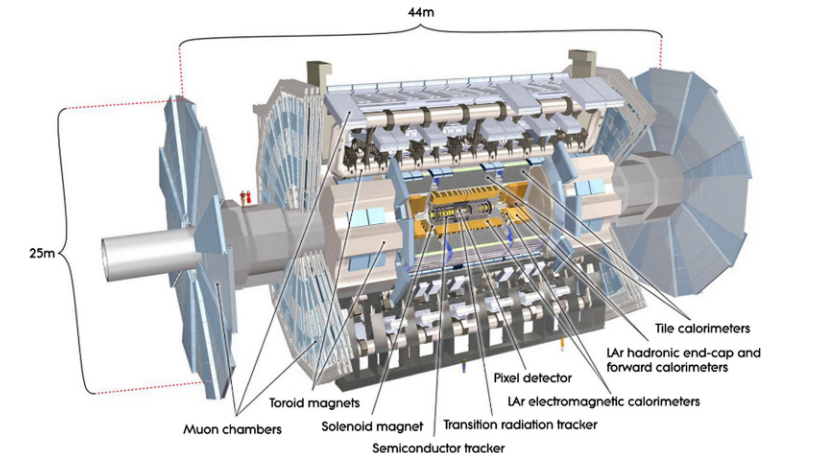
\includegraphics[scale=0.5]{chapter2/ATLAS.png}
\caption{Inner view of ATLAS detector,~figure taken from~\cite{Schott_2014}.}
\label{ATLAS_VIEW}
\end{figure} 

\begin{figure}[H]
\centering
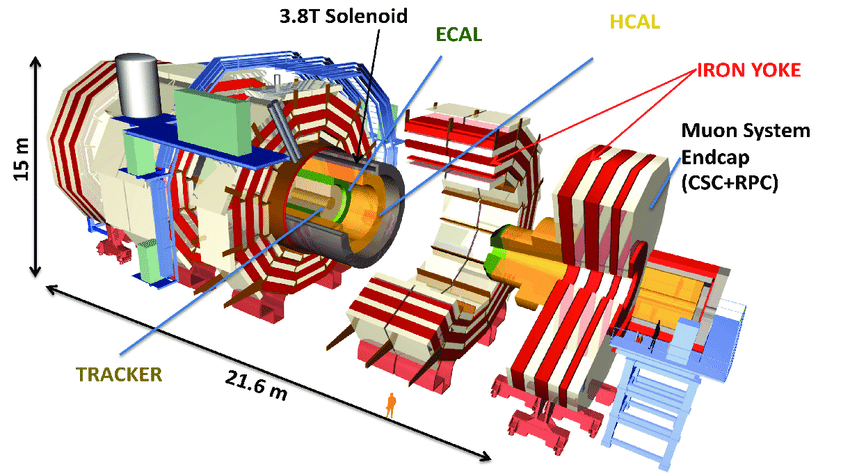
\includegraphics[scale=0.5]{chapter2/cms.png}
\caption{Schematic illustration of the CMS detector,~figure taken from~\cite{article11}.}
\label{cms1}
\end{figure}


\subsubsection{A Large Ion Collider Experiment~(ALICE)}
The ALICE~\cite{Collaboration_2008alice} is designed to study the properties of quark–gluon plasma, a rare state of matter. Quark-gluon plasma is the state of matter under very high temperature and densities in which quarks are free and not confined inside a hadron. 

\begin{figure}[H]
\centering
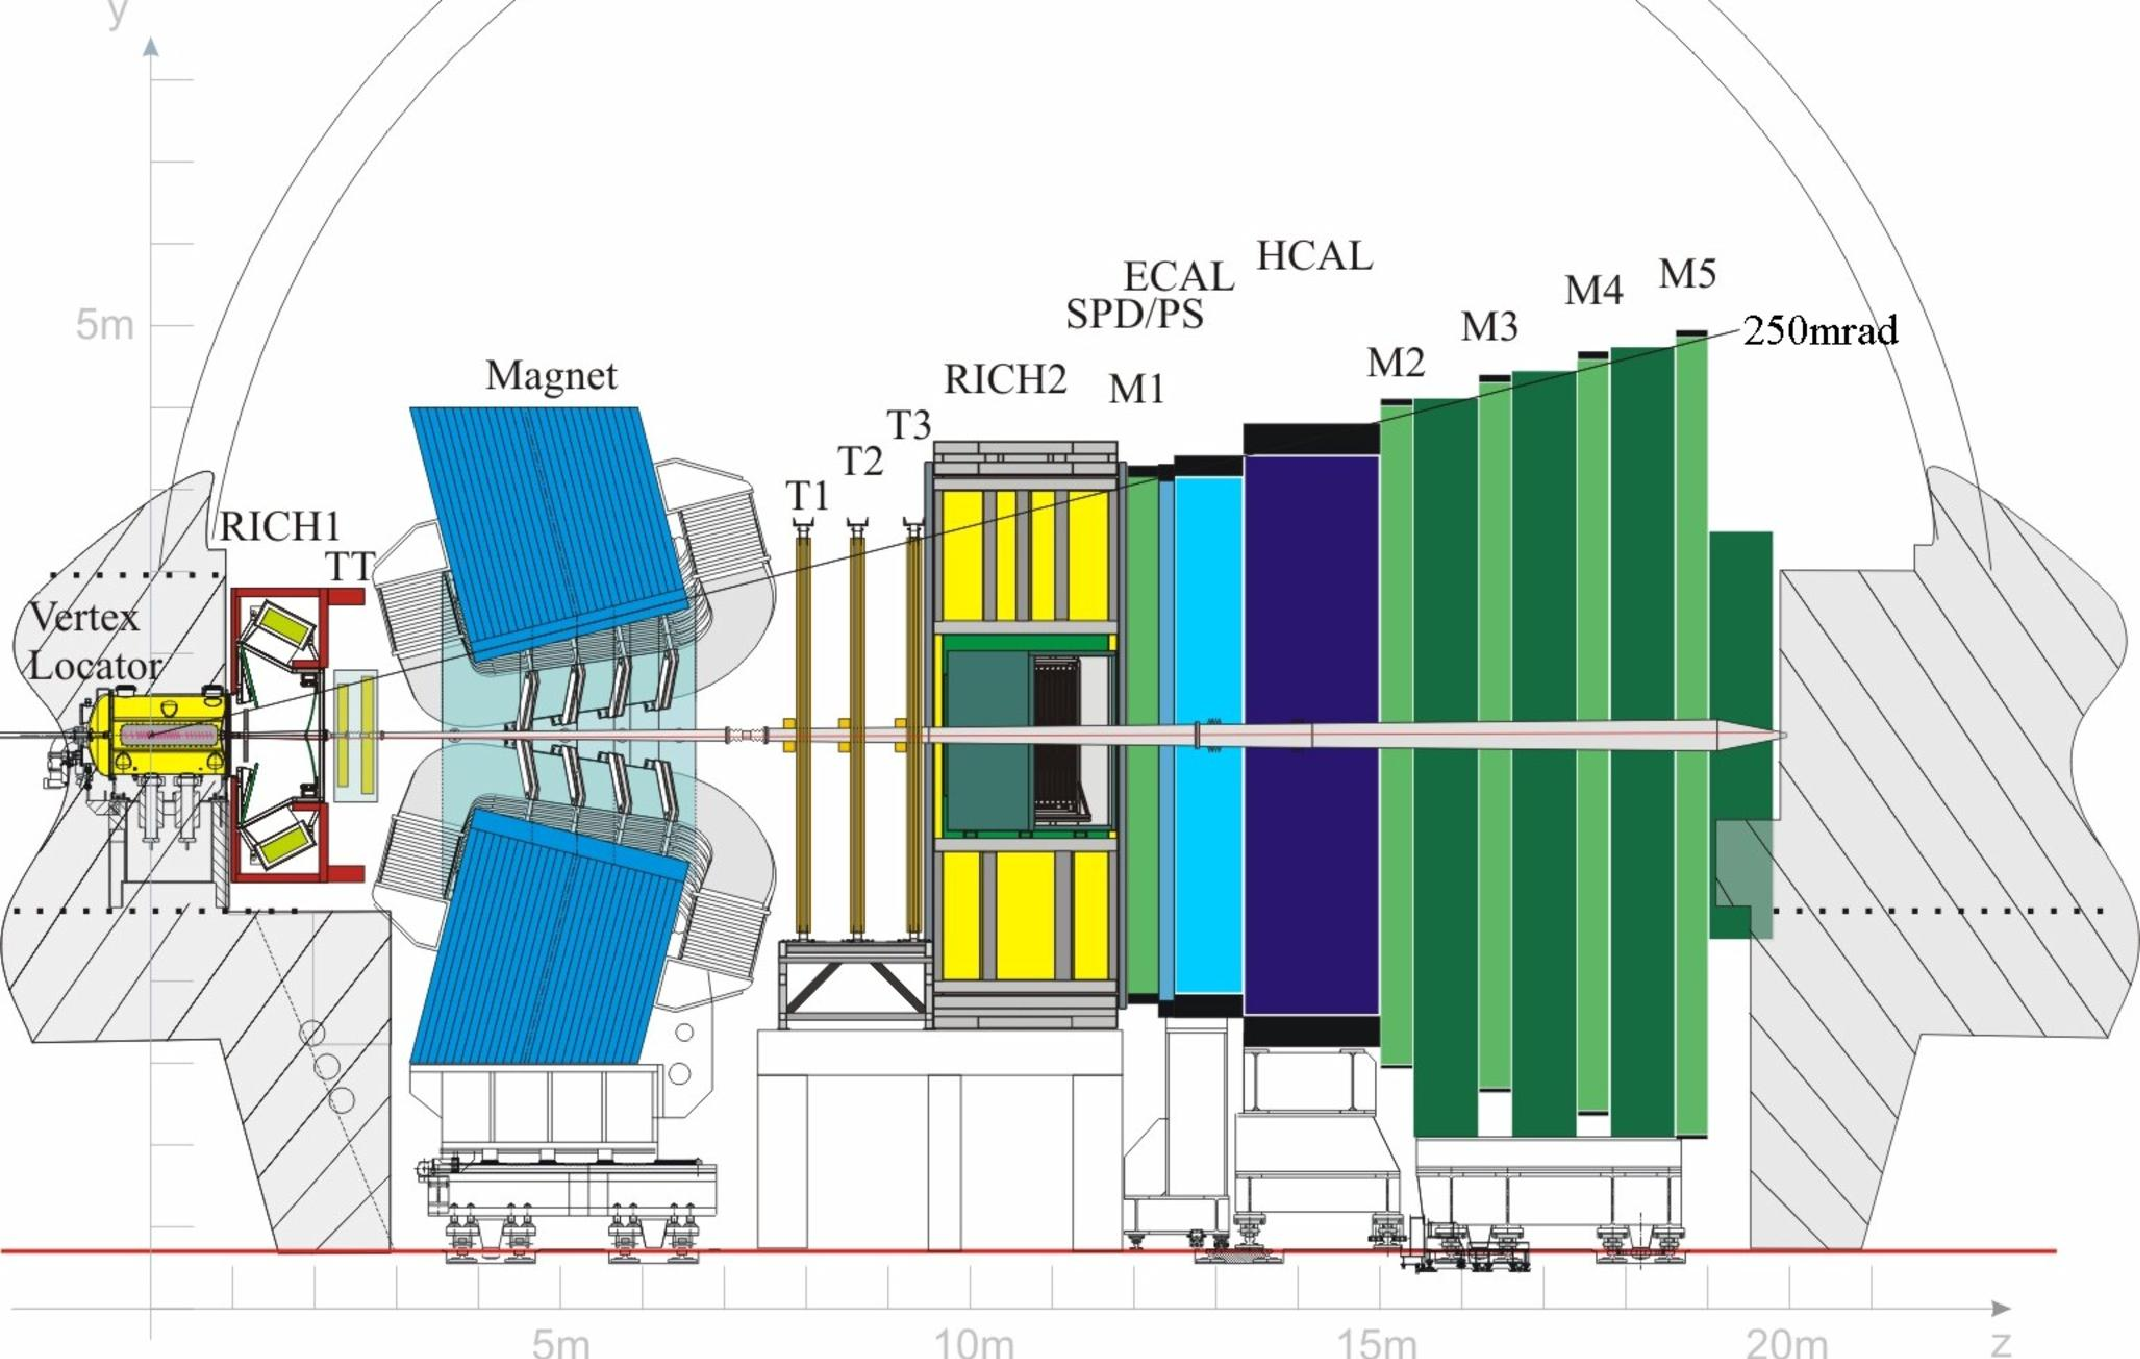
\includegraphics[scale=0.2]{chapter2/LHCb.png}
\caption{Inside view of the LHCb detector at LHC,~figure taken from~\cite{Mead:2780780}.}
\label{lhcb}
\end{figure}

\subsubsection{Large Hadron Collider Forward~(LHCf)}
The large hadron collider forward~(LHCf)~\cite{Collaboration_2008lhcf} is a small experiment that is designed to study different aspect of nuclear physics.

\subsubsection{TOTEM}
TOTEM~\cite{Collaboration_2008} is designed to measure the total cross section, elastic and diffractive scattering of the proton. TOTEM is able to detect particles that are produced very close to the beam pipe of LHC. The TOTEM is placed in a specially designed vacuum chambers called Roman pots. These Roman pots are connected to the beam pipes around LHC. There are total of 26 Roman pots in LHC which are located near CMS experiment as shown in Fig.~\ref{Totem}.

\begin{figure}[H]
\centering
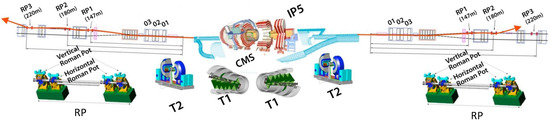
\includegraphics[scale=0.7]{chapter2/totem.jpg}
\caption{Sketch of the TOTEM and CMS experiments at the LHC~figure taken from~\cite{article}}
\label{Totem}
\end{figure}

\section{Parameters Of LHC}
\subsection{LHC Co-ordinate System}
The CMS and ATLAS detectors work using the right-handed cartesian system with center being the origin of the co-ordinates at the point where the interaction takes place. The $x-axis$ is directed towards the center of the hadron collider, the $y-axis$ is directed in the upward direction that is perpendicular to the ground whereas the third $z-axis$ is parallel to the proton beam, as shown in Fig.~\ref{co-ordinate lhc}. The polar angle, $\theta$, is the angle measured w.r.t the beam axis. The azimuthal angle, $\phi$, is the angle between the x-y planes. The distance $\Delta r$ between two particles is defined in the $\eta-\phi$ plane as
\begin{equation}
\Delta r = \sqrt{\Delta \eta^{2}+\Delta \phi^{2}}
\end{equation}
where $\Delta \eta=|\eta_{a}-\eta_{b}|$, $\Delta\phi=|\phi_{a}-\phi_{b}|$ and $\eta, \phi$ are polar and azimuthal angle of the particle tracks.
\begin{figure}[H]
\centering
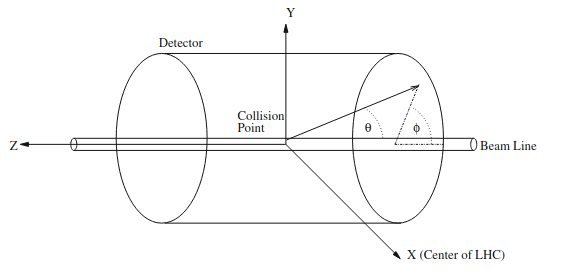
\includegraphics[scale=0.6]{chapter2/coordinate.png}
\caption{ATLAS and CMS coordinate system,~figure taken from~\cite{Schott_2014}}
\label{co-ordinate lhc}
\end{figure}
\subsection{Pseudo rapidity}
In hadron collider physics, a useful term defined as rapidity of the particle is given as
\begin{equation}
y=\frac{1}{2}ln\frac{E+p_{z}}{E-p_{z}} 
\end{equation}
where $p_{Z}$ is the momentum of particle along $z-axis$. The term pseudo rapidity '$\eta$' is derived from rapidity,~commonly measured in polar angle $\theta$ with respect to beam axis. Pseudo rapidity is defined by the equation $\eta=-\ln(\tan\frac{\theta}{2})$.
\begin{figure}[H]
\centering
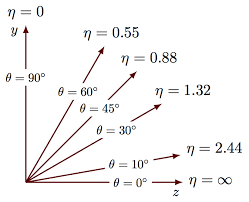
\includegraphics[scale=0.6]{chapter2/pseudorapidity.png}
\caption{Pseudo rapidity values in $1^{st}$ quadrant}
\end{figure}
where '$\theta$' is the angle between particle direction and beam direction.  The transverse momentum '$p_{T}$' is defined as the component of particle momentum in x-y plane. The transverse energy is defined as $E_{T} =
E sin\theta$.

The energy which is carried by non detectable particles is called missing energy, because these particles have no interaction through strong or electromagnetic forces, these particles are called neutrinos. In general, missing energy arises due to presence of non-detectable particles in the detector. The particle travelling in transverse direction to the beam axis have zero initial momentum, so if we have final momentum in $x$ or $y$ direction, it represents the missing transverse energy, because the total transverse momentum of initial state is zero, sum of final state particle’s transverse direction should also be zero. Missing transverse momentum~\cite{PortilloQuintero:2668716} can be defined by following equation,
\begin{equation}
\overrightarrow{E}_{T}^{missing}=-\Sigma_{i}\overrightarrow{p}_{T}^{i}
\end{equation}
Where, the index $i$ sums over all visible particles. The assumption that transverse energy and momentum are equal, holds only for particles that are massless.
The missing transverse momentum is defined as
\begin{equation}
\overrightarrow{p}_{T}^{missing}=-\Sigma_{i=1}^{N}\overrightarrow{p}_{T_{i}}
\end{equation}
In an event $N$ is the total number of final state particles. The $p_{T} $ and $p_{T}^{missing}$ are invariant under Lorentz boost along the beam direction which is $z-axis$. 
For particles of mass very smaller than their energy $(m<<E)$ the rapidity can be approximated by pseudo rapidity $\eta$.
\subsection{Luminosity}
Luminosity~\cite{Aberle:2749422} is a important parameter of the accelerator. To observe new phenomena in experimental high energy physics, we required high center of mass energy such as up to $14~TeV$, as well as large number of useful interactions. These useful interactions are used to reconstruct data for the analysis. In the study of rare events with very small cross section $\sigma$, luminosity becomes more important. The total number of interactions that an accelerator can produce is called its luminosity and it is the proportionality factor between event production rate $\frac{dR}{dt}$ and the cross section $\sigma$:
\begin{equation}\label{ins-lumi}
\frac{dR}{dt}=\mathcal{L}_{ins}.\sigma
\end{equation}
Luminosity can be defined simply by, ratio of the number of events produced~$(dN)$ in a certain time~$(dt)$ to cross section $\sigma$. 
\begin{equation}\label{ins-lumi}
\mathcal{L}_{ins}=\frac{dN}{\sigma dt}
\end{equation}
 
The unit of luminosity is $cm^{-2}s^{-1}$. The rate of collisions also relate to instantaneous luminosity $\mathcal{L}_{ins}$ as:
\begin{equation}\label{in_lumi}
N=\mathcal{L}_{ins}\times\sigma
\end{equation}
Where $\sigma$ is cross section of expected process. Equation~\ref{in_lumi} shows that the instantaneous luminosity cannot be kept stable during the data taking~\cite{Waqas:2779481}. $\mathcal{L}$ decreases due to loss of protons in bunches, which leads to decrease in collision rate. Therefore, another useful quantity in detector physics integrated luminosity~$\mathcal{L}_{int}$ is introduced by integrating the instantaneous luminosity over time, having units inverse barns denoted by $b^{-1}$ (per $cm^{2}$). It is used to measure how much data is recorded by LHC and CMS.\\
The data acquisition system  of detector is not always 100~$\%$ efficient due to which the amount of data recorded by a detector is usually smaller than the amount of data delivered, and not all the data is good enough for analysis purpose, as some of the subsystems may be in an error state that corrupt the data recorded or other unexpected behaviour of the LHC or CMS may have interrupted the data recording. The total amount of data used in an analysis can be much smaller than the total amount of data delivered. Fig.~\ref{CMS_lumi} shows the predicted increase in luminosity of CMS detector with center of mass energy.
\begin{figure}[H]
\centering
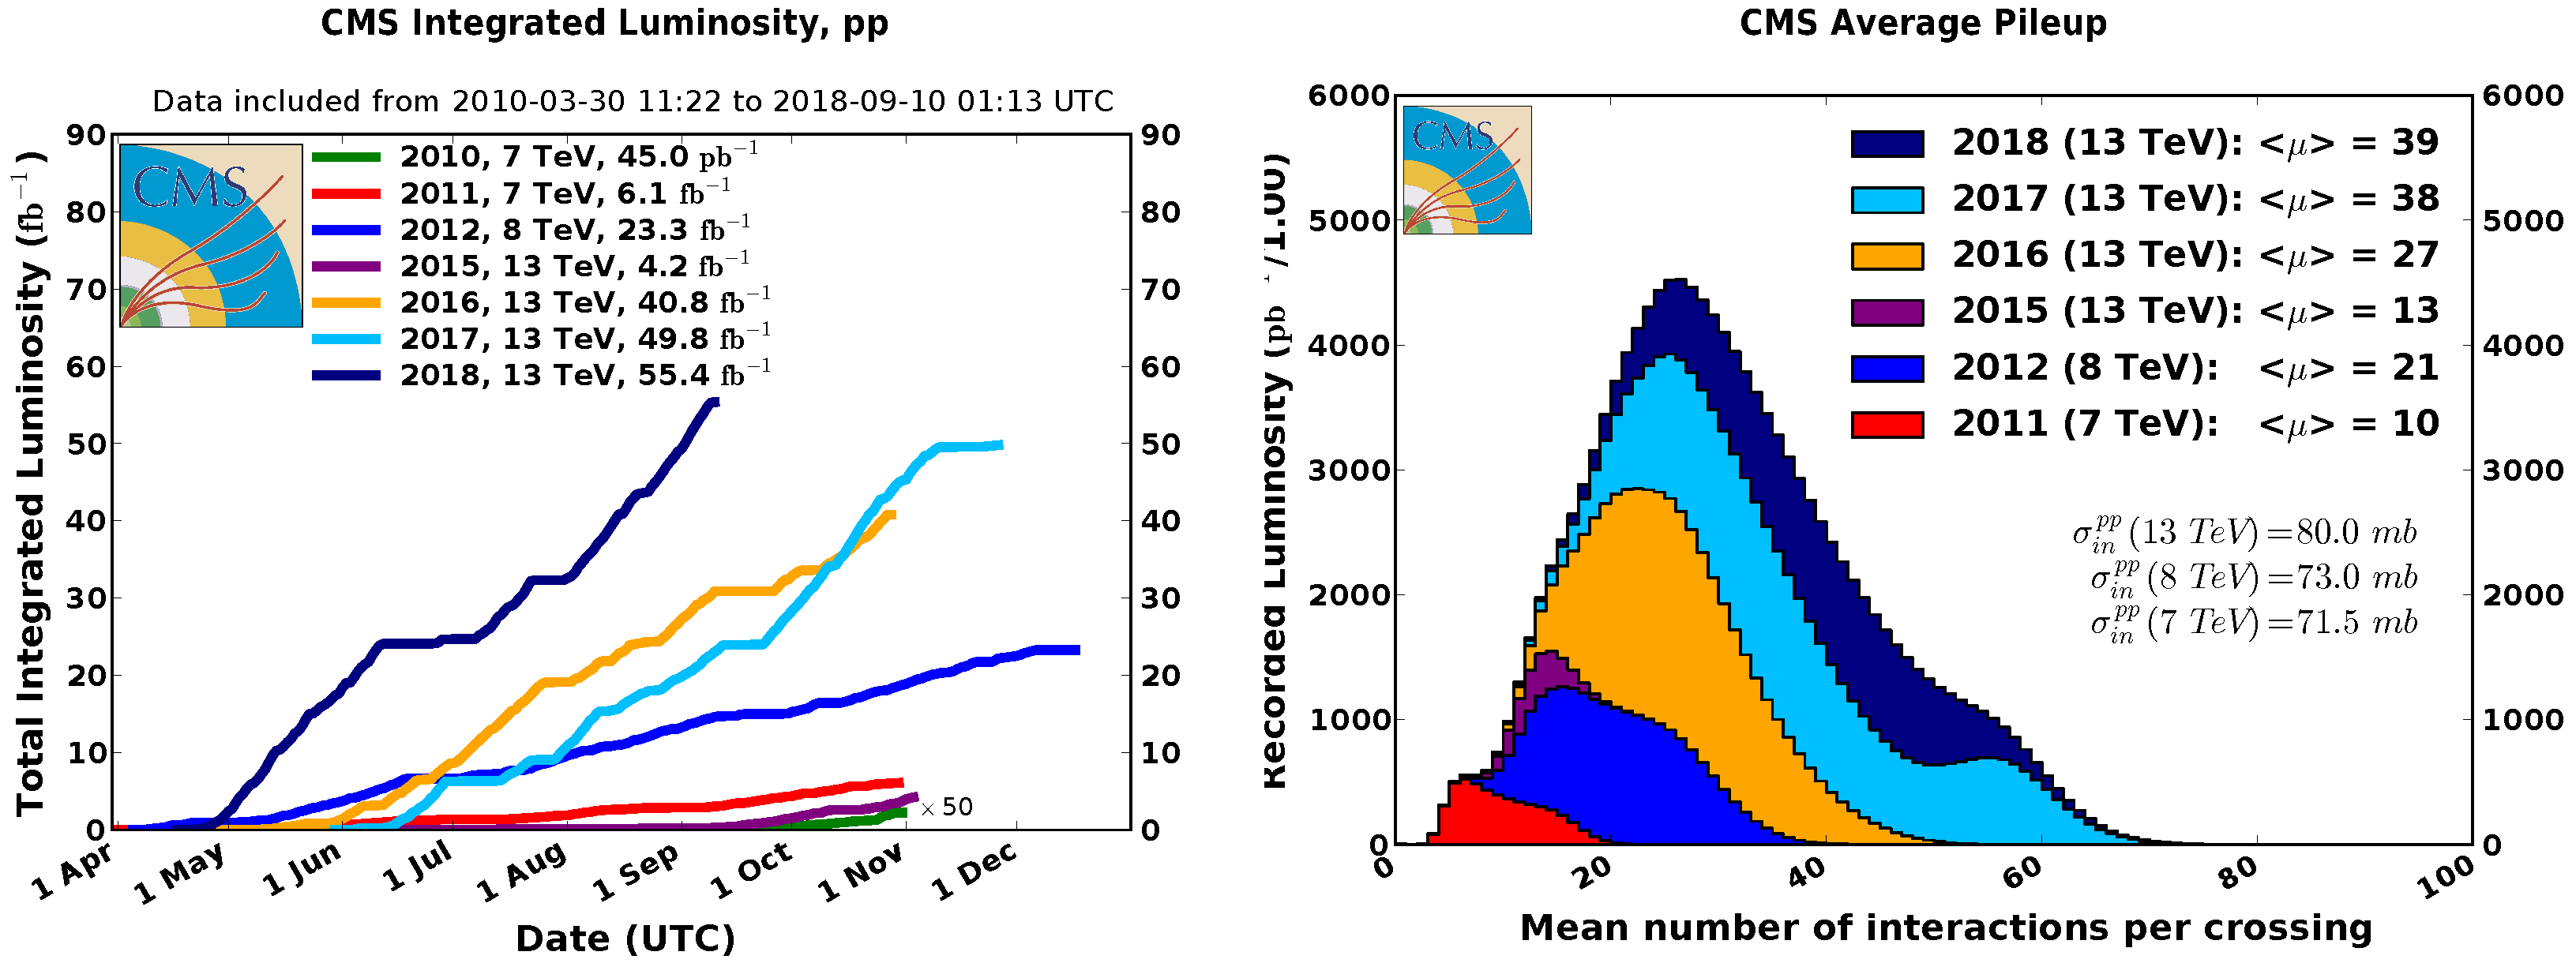
\includegraphics[scale=1]{chapter2/cms-lumi.png}
\caption{$\mathcal{L}_{int}$ delivered to CMS versus data taking period for pp collisions at different LHC energies. The distribution of $<\mu>$ versus luminosity recorded by CMS for the 2011~-~2012 and 2015~-~2018 data taking period~figure adopted from~\cite{Aberle:2749422}. }
\label{CMS_lumi}
\end{figure}
\subsection{Pile-up (PU)}
Another important parameter of the accelerator is pileup. During a bunch crossing multiple proton-proton interactions can occur which are referred to as pileup. These interactions are proportional to the event cross section times luminosity. There are two types of pileups:
\begin{itemize}
\item in-time PU comes from the collisions happening in the same bunch crossing.
\item out-of-time PU comes from the collisions from the previous bunch crossings whose signal has not yet been recorded by the detector.
\end{itemize}
In-time PU is calculated by the number of primary vertices ($N_{PV}$ ) while out-of-time PU is parametrized by the mean number of interactions per bunch crossing ($\mu$). In 2012 an average of 21 pileup interactions was observed at $8~TeV$. This increased in 2016 due to the higher luminosity and cross section at $13~TeV$, to about 27 interactions on average. 


\subsection{Beam Spot}
This spot is the brightest region where the two beams travelling in opposite direction are brought into collision. It is an important and an essential parameter for the computation of different parameters which are used in further data analysis. It is very necessary to measure beam spot very accurately and precisely, especially the beam spot width, the value of beam spot width is further used by computation procedure of different observables. It is also a reference point for studying the track performance.

\section{CMS Detector}
The Compact Muon Solenoid (CMS)~\cite{Collaboration_2008cms}, as the name represents is compact due to small size when compared to ATLAS detector, muon is a fundamental particle detected by CMS, and solenoid for the large superconducting magnet. The side view of CMS detector is shown in Fig.~\ref{CMS_sideview}. The scientific goals of CMS experiment are same as for the ATLAS. After the discovery of Higgs boson, the study of Higgs boson properties in detail and search for the physics beyond the Standard Model are the main goals of CMS experiment. CMS has a different technical solution, especially its magnetic system design.\\
The CMS detector built $100m$ underground in France countryside, near the village of Cessy. One of the main goals to built CMS experiment was the search of Higgs boson that is responsible of electroweak symmetry breaking. This goal was achieved in $2012$ by the discovery of scaler boson named "SM Higgs Boson"~\cite{Chatrchyan_2012}. CMS experiment covers many aspects of proton-proton collisions at very high center of mass energy i.e.~($14~TeV$) of the LHC. 
Some of the main characteristics of CMS are as follows:
\begin{itemize}
\item CMS provides a better muon identification and momentum measurement over wide range of angle.
\item CMS tracking system provides good identification of the charged particles.
\item A wide geometric coverage, better electromagnetic energy resolution.
\end{itemize}
\subsection{Structure of CMS}
The CMS detector has a long cylinder of length $21.6~m$ with a diameter of $15~m$ and weight $12500~tons$. It is designed to operate at a center-of-mass energy of $14~TeV$ and a luminosity of $10^{34}~cm^{-2}s^{-1}$. The CMS uses superconducting solenoid magnet that surrounds all the inner detectors. CMS is equipped with different types of silicon tracker,~i.e., silicon pixel and strip tracker, lead-tungstate~$(PbWO_4)$ Electromagnetic Calorimeter and a brass scintillator sampling Hadronic Calorimeter. An iron yoke which holds both superconducting solenoid and muon detector.\\ 
CMS has also right handed coordinate system, with the origin at the interaction point of beam inside the detector. CMS has cylindrical symmetry, it is convenient to use cylindrical co-ordinates $(r,\theta,\phi)$ shown in figure~\ref{cms-polar}.\\
The CMS structure can be summarized as below:
\begin{itemize}
\item The interactions between bunches of particles take place at the core of the apparatus with a maximum instantaneous luminosity of $21~nb^{-1}s^{-1}$ achieved in LHC RUN 2.
\item The inner part of detector is silicon tracker which extend from interaction point to $|r|<1.2m$, covering $|\eta|$ range $<2.5$.
\item The Electromagnetic calorimeter~(ECAL) extends over $1.2m < r < 1.8m$ and covers pseudo-rapidity range $|\eta|<1.3$.
\item The Hadronic Calorimeter~(HCAL) covers $1.8~m < r <2.9~m$ by covering $|\eta|<5$.
\item The superconducting solenoid magnet provides a magnetic field of $4~T$ along the beam direction, which bends the charged particles trajectories in order to measure their momentum. The solenoid surrounds all the inner detectors and extends from $2.9~m < r < 3.8~m$ over $|\eta|<1.5$. 
\item The muon system is the outer most part of the CMS detector. It is extended from $4~m < r < 7.4~m$ and covers $|\eta|<2.4$.
\end{itemize}
\begin{figure}[H]
\centering
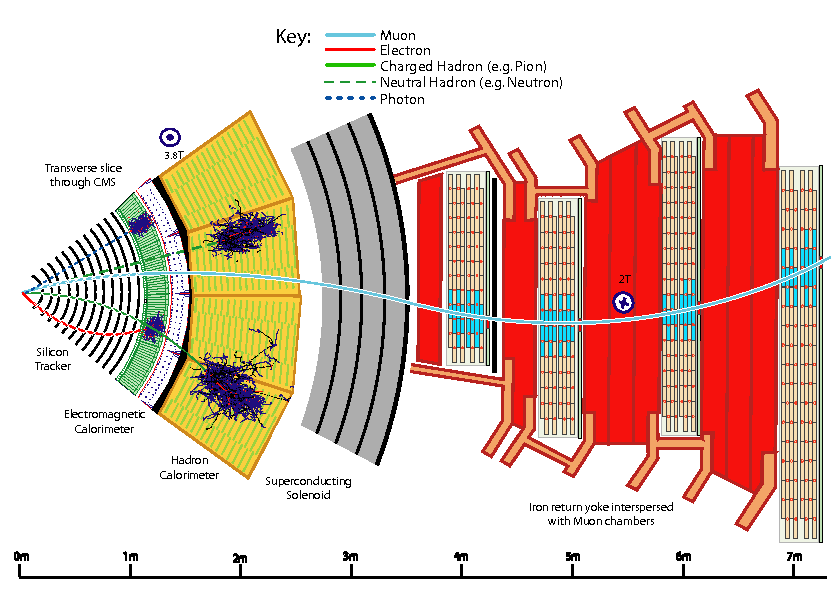
\includegraphics[scale=0.5]{chapter2/CMS_cutview.png}
\caption{Cut view of CMS detector, the distance of different components from center is illustrated in figure taken from~\cite{Davis:2204863}}
\label{CMS_sideview}
\end{figure}

\begin{figure}[H]
\centering
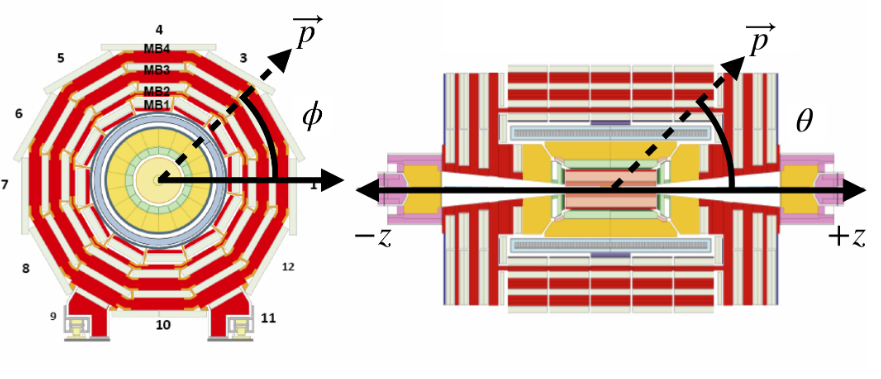
\includegraphics[scale=0.48]{chapter2/cms-coordinate.png}
\caption{Polar coordinates used by CMS. Figure taken from reference~\cite{Collaboration_2010}.}
\label{cms-polar}
\end{figure}


\subsection{CMS Tracker}
The tracker is located very close to the interaction point as shown in Fig.~\ref{CMS_schematic} hence it receives the largest number of particles produced. The tracker is designed to measure highest resolution of charged particles trajectories with transverse momentum up to $1~GeV$ in a range $|\eta|=2.5$. At LHC 
design luminosity of about $10^{34}~cm^{-2}s^{-1}$, the tracker records roughly 100 tracks per bunch crossing,~i.e., for every $25~ns$. So it is necessary to choose the construction material carefully to resist high radiation and particle flux.
\begin{figure}
\centering
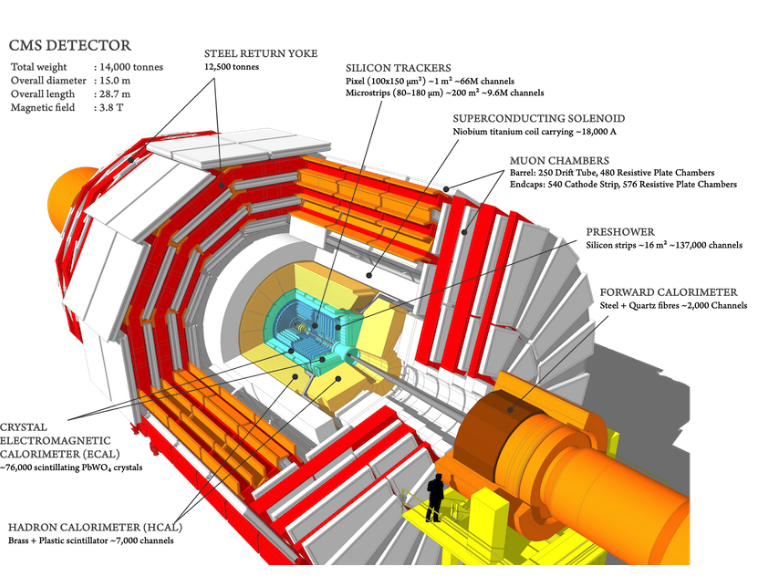
\includegraphics[scale=0.5]{chapter2/cms-schematic.png}
\caption{Schematic view of CMS detector. Figure taken from~\cite{Layter:343814}.}
\label{CMS_schematic}
\end{figure}

\subsection{Electromagnetic Calorimeter~(ECAL)}
The ECAL~\cite{CERN-LHCC-97-033} sits in between the tracker and Hadron Calorimeter~(HCAL). It is designed to detect and measure the energy of photons, electrons and positrons with great precision. There are three partitions in ECAL: Barrel, End caps and Pre shower. The ECAL barrel~(EB) has $61200$ $PbWO_{4}$ crystals, in a cylindrical shape design that begins at a radius of 1.29~m  and covers the range $|\eta| < 1.479$. The barrel has a number of module and super module. The barrel region is complemented by $7324$ crystals that are mounted on two end caps located at 314~cm from the vertex and cover the range $1.47 < |\eta| < 3.0$.\\
The pre shower detector is placed in front of the end cap crystal and covers a range of $1.653 < |\eta| < 2.6$. It discriminates the electromagnetic shower formed by the photons, coming from the neutral pion decay. It also helps to identify the position of electrons and photons. The layout of ECAL can be seen in Fig.~\ref{ecal1}.

\subsection{Hadron Calorimeter~(HCAL)}
The Hadron Calorimeter~\cite{collaboration_2011} is designed for the study of many processes, which include energy and direction of hadronic jets, reconstruction of the hadron decays and missing transverse energy in the events. There are four modules of HCAL, the hadron barrel~(HB), hadron calorimeter end caps~(HE), the outer calorimeter~(HO), and the forward calorimeter~(HF).\\
The hadron barrel~(HB) shown in Fig.~\ref{hcal1} sits in between ECAL and superconducting magnetic coil at a distance $1.77~m < r < 2.95~m$. The hadron calorimeter end caps~(HE) cover the solid angle between $ 1.3 < |\eta| < 3$. The hadron barrel~(HB) calorimeter measures $860~cm$ in length with inner and outer radius of $177~cm$ and $295~cm$ respectively. HB is divided into two half-barrel HB+ and HB-. The end caps of HE cover range $1.3 < \eta < 3.0$. The HB+ and HB- have thirty six identical wedges. Each wedge is constructed from flat steel and brass plate and is aligned parallel to beam axis. The HE is also radially divided into 14 rings. The HO of HCAL is made with plastic scintillator in several layers and the most outer part of HCAL is HO which is $11.2~m$ away from the  collision point. 
\begin{figure}[H]
\centering
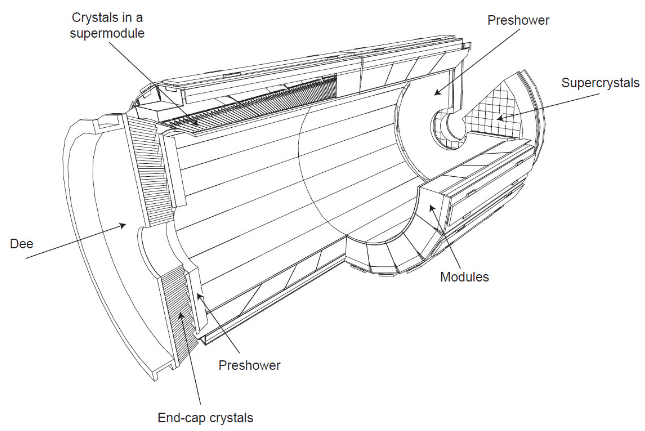
\includegraphics[scale=0.5]{chapter2/Ecal1.png}
\caption{CMS ECAL layout,~figure taken from~\cite{Collaboration_2008cms}.}
\label{ecal1}
\end{figure}
\begin{figure}[H]
\centering
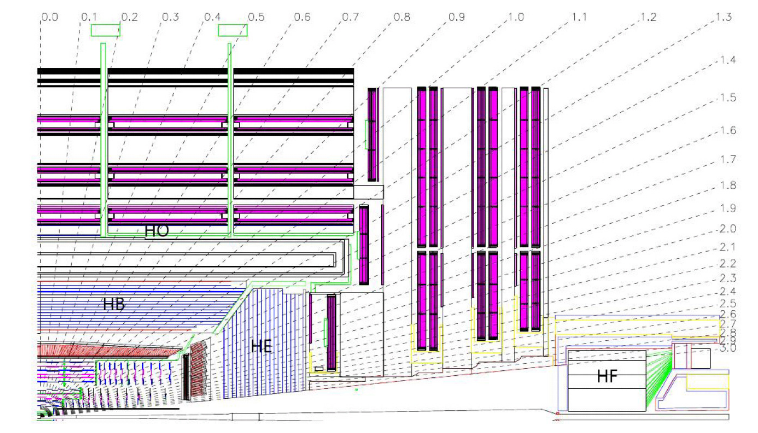
\includegraphics[scale=0.5]{chapter2/Hcal1.png}
\caption{Layout of CMS HCAL,~figure taken from~\cite{Collaboration_2008cms}.}
\label{hcal1}
\end{figure}

\subsection{Magnetic System of CMS}
The distinct feature of CMS is its superconducting magnet~\cite{Klyukhin:2773274} designed to provide magnetic field of $4~T$ in a region of length $12.5~m$ and $6~m$ in width, one of the biggest solenoid ever made.\\
In CMS detector we need high magnetic field to bend particle trajectories which is obtained by combination of different magnets made by NbTi cables. The energy stored at an operating temperature of $4.6~K$ and at full current is $\approx$ ~$2.6~GJ$. The magnetic flux of these coils is returned through an iron yoke weighing $10,000~tons$. It is shown in Fig.~\ref{CMS_magnet}. 

\begin{figure}[H]
\centering
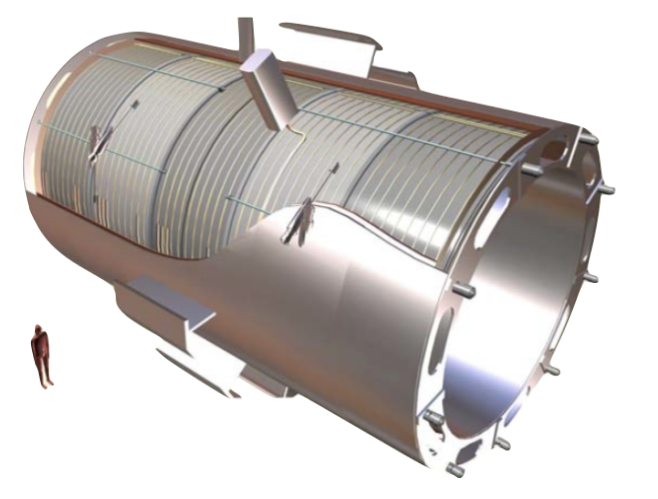
\includegraphics[scale=0.5]{chapter2/magnetic-cms.png}
\caption{View of CMS superconducting solenoid. Figure adopted from~\cite{Collaboration_2008cms}.}
\label{CMS_magnet}
\end{figure} 

\subsection{CMS Muon System}
The CMS muon system~\cite{Sirunyan_2018} is specially designed to detect muons with high transverse momentum. Its main function is to identify muon, measurement of its momentum and triggering.\\
The muon system of CMS is divided into three independent subsystems, which consist of three gaseous particle detectors, the drift tube system, cathode strip chambers and the resistive plate chambers.\\
\subsubsection{Drift Tube Chamber}
The barrel region of CMS muon system is instrumented with drift tube~(DT) chambers covering the pseudo-rapidity range up to $|\eta|~=~1.2$. The DT chambers arranged into five iron wheels, each wheel have four concentric ring called stations. The function of these stations is to measure the muons coordinates in the transverse plane as well as its $z$ direction.\\
The detector of this chamber is a drift tube of rectangular shape of size $ 13\times42~mm^{2}$ and having length $2-4~m$. The whole volume is filled with gas mixture of $85\%$ argon and $15\%$ carbon dioxide.\\
\subsubsection{Cathode Strip Chamber}
The cathode strip chamber is installed at the end cap of CMS muon system. This chamber is designed especially to identify muons in the region $0.9 < |\eta| <  2.4$. The chamber is divided into four stations for each end cap, perpendicular to the beam pipe and separated by the flux return plate as can be seen in Fig.~\ref{csc1}.\\ 
\begin{figure}[H]
\centering
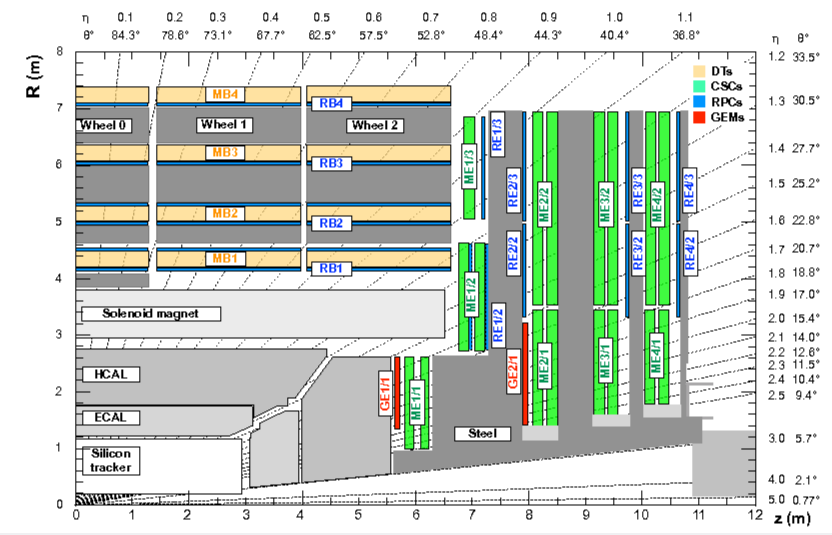
\includegraphics[scale=0.5]{chapter2/csc1.png}
\caption{CMS muon detector system. Figure adopted from~\cite{Sirunyan_2018}.}
\label{csc1}

\end{figure}
The cathode strip chamber is filled with $40\%$ argon and $50\%$ carbon dioxide as active gas and remaining $10\%$ with carbon tetrafluoride. This chamber is arranged in four disks called stations, each of which has two rings divided into eighteen or thirty six CSCs. These stations are equipped with sensitive wires which provide muon recognition.

\subsubsection{Resistive Plate Chamber}
The resistive plate chambers~(RPC) are installed at both barrel and end cap regions. They are also gaseous detector. The RPCs are made of four Bakelite planes coated with graphite which act as the electrode and two gas gaps of $2mm$.\\

\subsection{CMS Trigger System}
LHC provides proton-proton and heavy ions collisions at a very high rate as shown in Fig.~\ref{recoreder_lumi}. High particle density in each bunch corresponds to an event rate of 40 MHz with 20 head-on collisions per event, thus interaction rate exceeds 1~GHz. Such a high data stream cannot be handled with current available technology. Therefore, CMS experiment uses a dedicated trigger system. The trigger system selects possible events of interest among all the simultaneous events occurring.\\
The trigger system~\cite{Khachatryan_2017} is divided into two main stages:\\
\begin{enumerate}
\item Level-1 trigger~(L1) system consists mainly of programmable electronic components.
\item High Level Trigger~(HLT) system is fully software based.
\end{enumerate} 
The L1 trigger preselects events of interest in order to be further analysed by the HLT. L1 trigger is responsible for the identification of different leptons, quark jets and missing transverse energy. It consists of three main subsystems:
\begin{itemize}
\item Calorimeter Trigger
\item Muon Trigger
\item Global Trigger
\end{itemize}  

\begin{figure}[H]
\centering
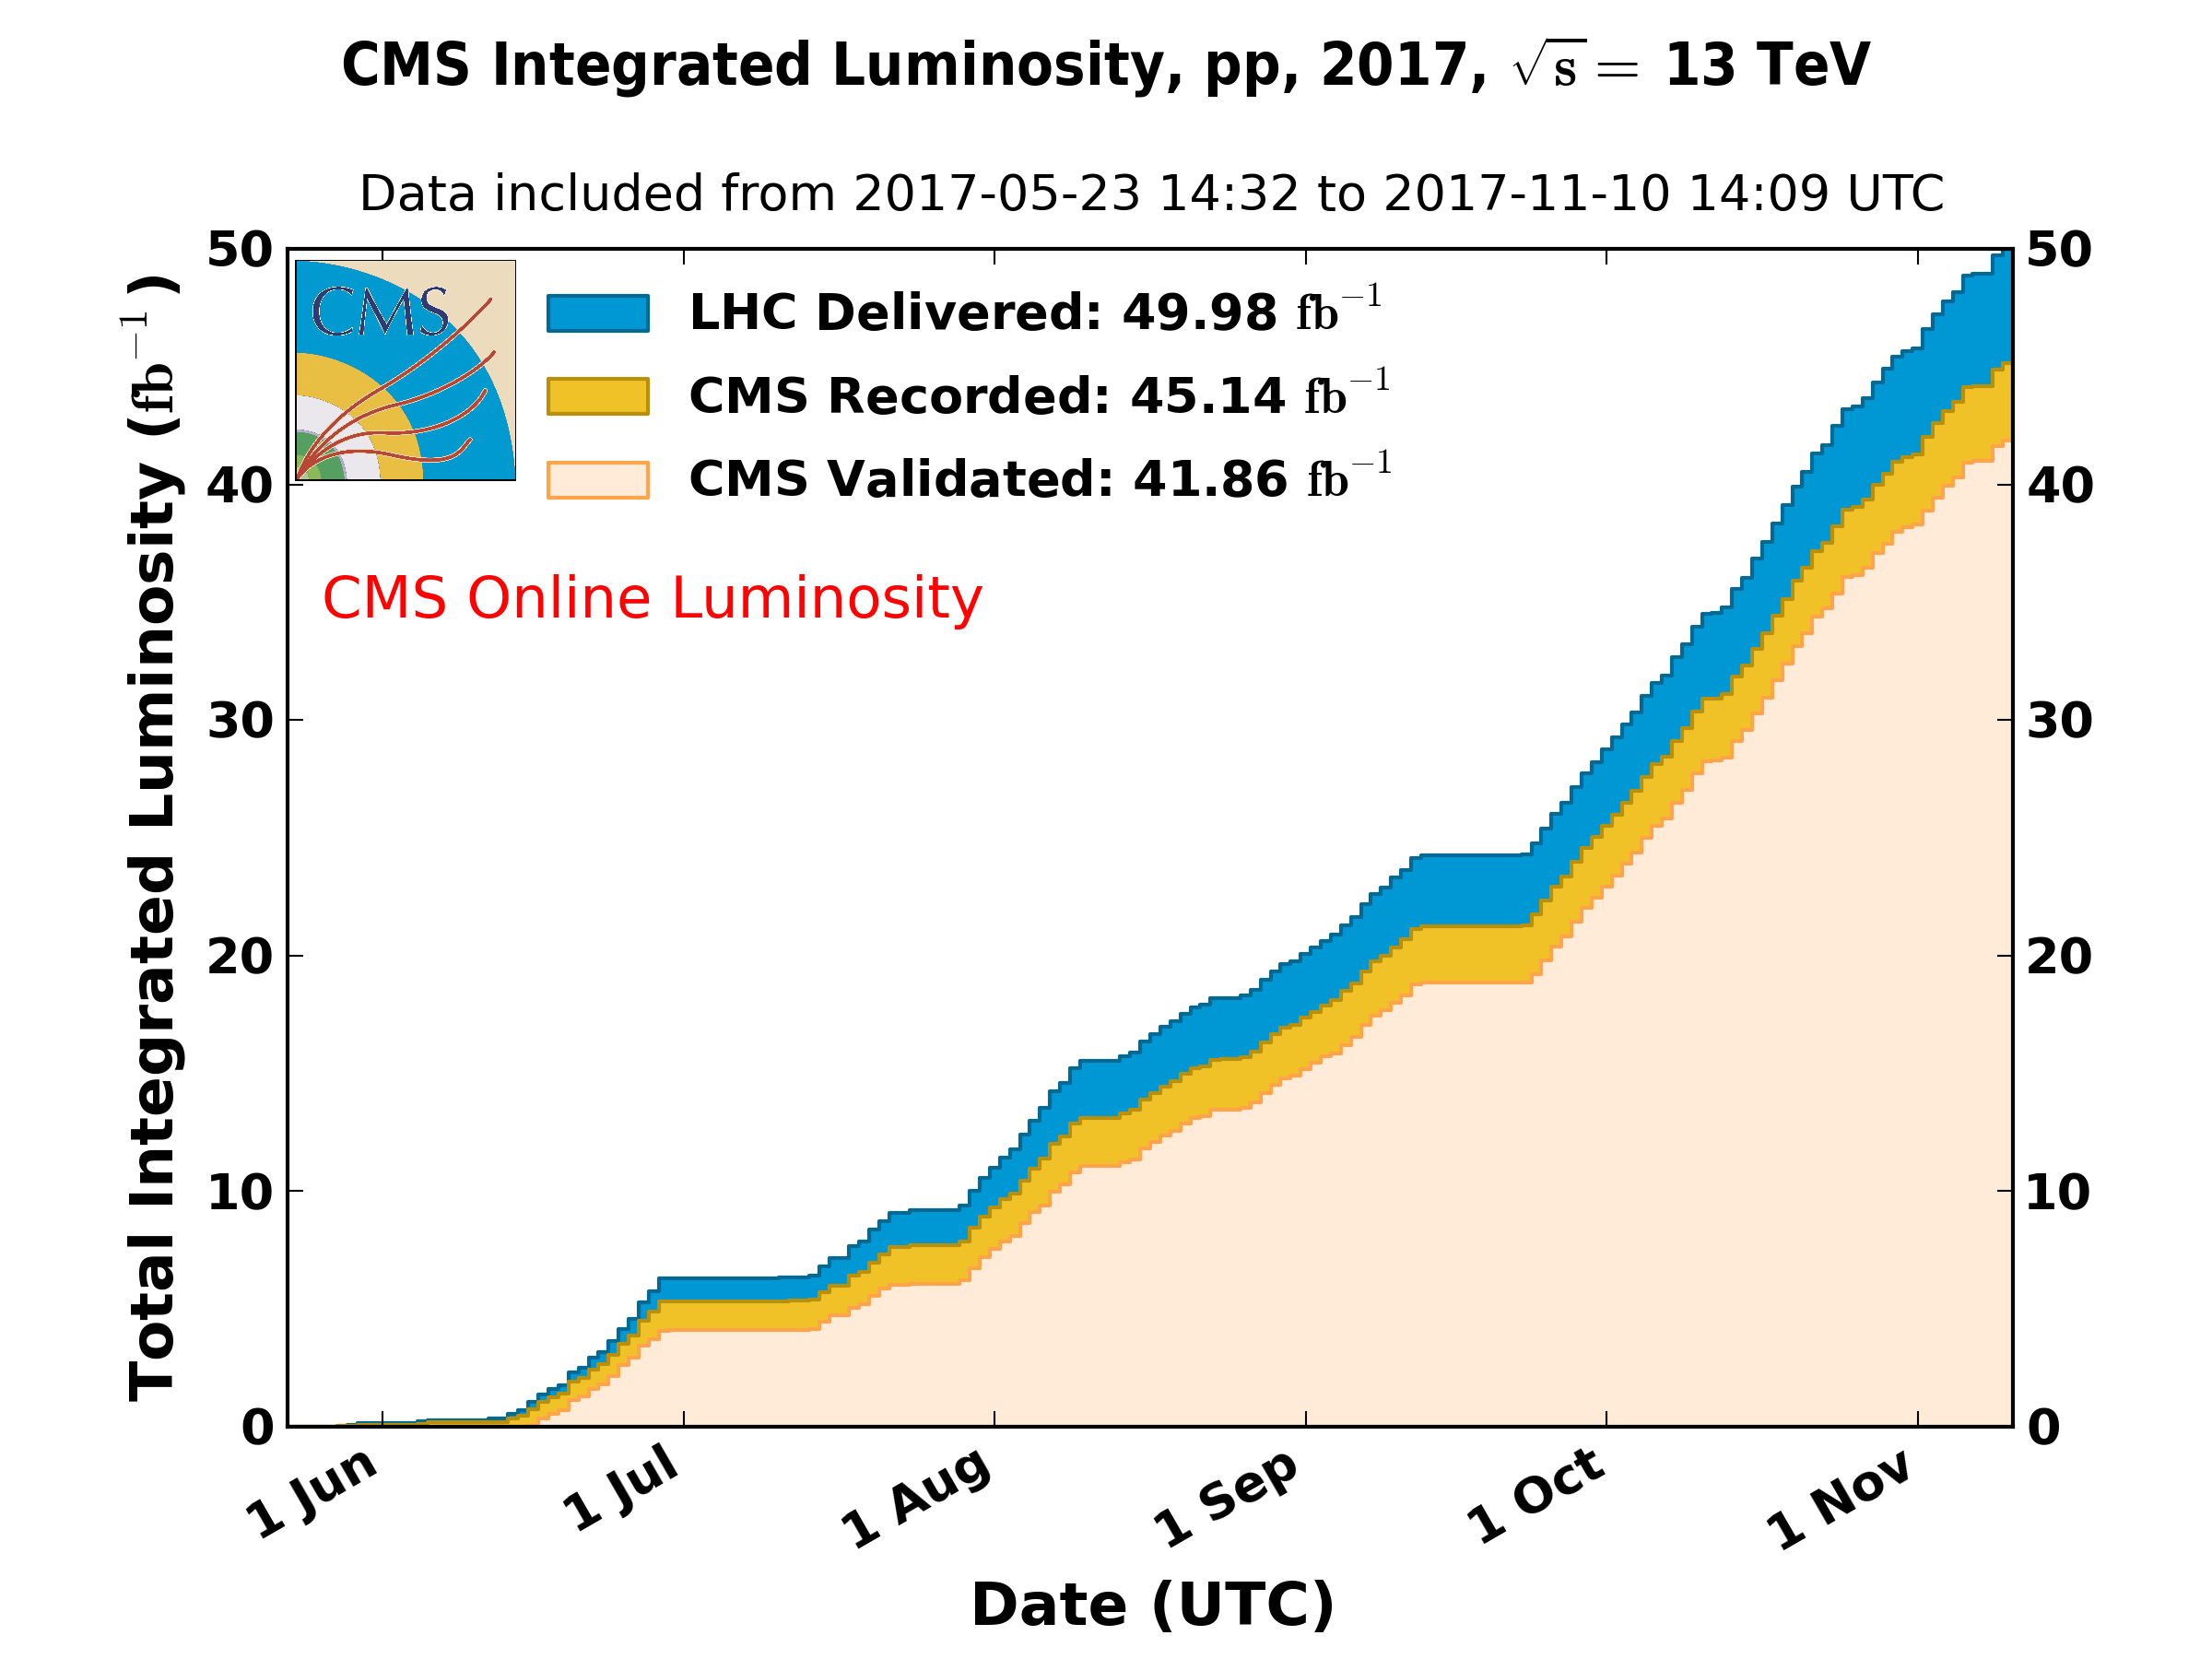
\includegraphics[scale=0.5]{chapter2/cms luminosity.png}
\caption{CMS recorded luminosity at $13~TeV$.}
\label{recoreder_lumi}
\end{figure} 


The event selection at the \textbf{HLT}~\cite{Cittolin:578006} is similar to that used in the offline processing. HLT reconstructs the leptons, jets and applys the identification criteria in order to select only those events which are of possible interest for data analysis. A view of the CMS L1 trigger is shown in Fig.~\ref{cms-trigger}.

\begin{figure}[H]
\centering
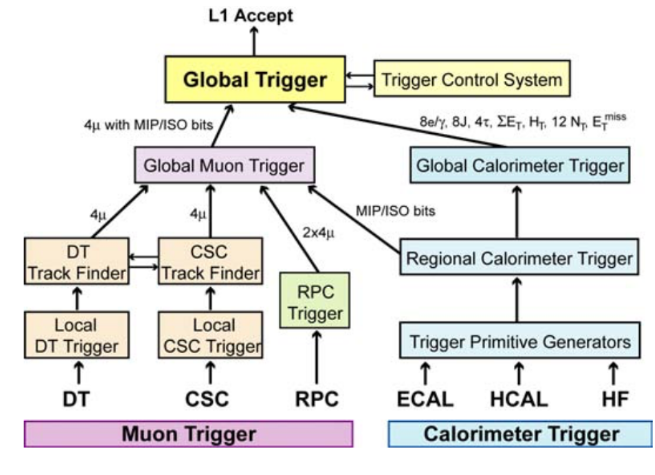
\includegraphics[scale=0.5]{chapter2/cms-trigger.png}
\caption{The L1 trigger system of CMS,~figure taken from~\cite{Collaboration_2008cms}.}
\label{cms-trigger}
\end{figure} 


